\documentclass{article}
\usepackage{graphicx}
\usepackage{cmap}
\usepackage[russian]{babel}
\usepackage[utf8]{inputenc}
\begin{document}
\begin{center}
\large{Сравнение алгоритмов классификации на предмет устойчивости к зашумлению входных данных}
\end{center}
\newpage
\section{Постановка задачи}
Изобилие алгоритмов машинного обучения даёт определённый простор для выбора. К сожалению данные, предоставленные для обработки, зачастую содержат ошибки и неточности. Не секрет, что критериев такого сравнения можно придумать очень много, так почему бы не сравнить алгоритмы по устойчивости к порче входных данных? Для этого рассмотрим три популярных алгоритма: SVM, Decision Tree и Naive Bayes и рассмотрим их на датасете рукописных цифр, которые будем постепенно портить.
\section{Практическая часть}
В качестве датасета был выбран MNIST Database, так как изображения в нём подвегнуты качественному перпроцессингу и мы можем быть уверены, что изображение испортили именно мы. Портить изображение будем наложением случайных шумов. Ниже приведён пример.

\centering
\begin{figure}
	%\begin{subfigure}[b]{width=.3\textwidth}
	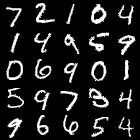
\includegraphics[width=.3\textwidth]{graphics/digits.jpg} 
	%\end{subfigure}
%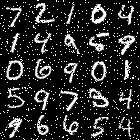
\includegraphics[width=.3\textwidth]{graphics/digits_spoiled10percent.jpg} &
%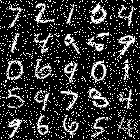
\includegraphics[width=.3\textwidth]{graphics/digits_spoiled20percent.jpg} 
%\caption{Пример зашумления изображений}
\end{figure}
\begin{itemize}
\item Запустить построение гипотезы на неиспорченных данных, а проверять гипотезу на испорченных данных
\item Строить гипотезу и проверять её на испорченных случайным образом данных(например, шум). 
\end{itemize}
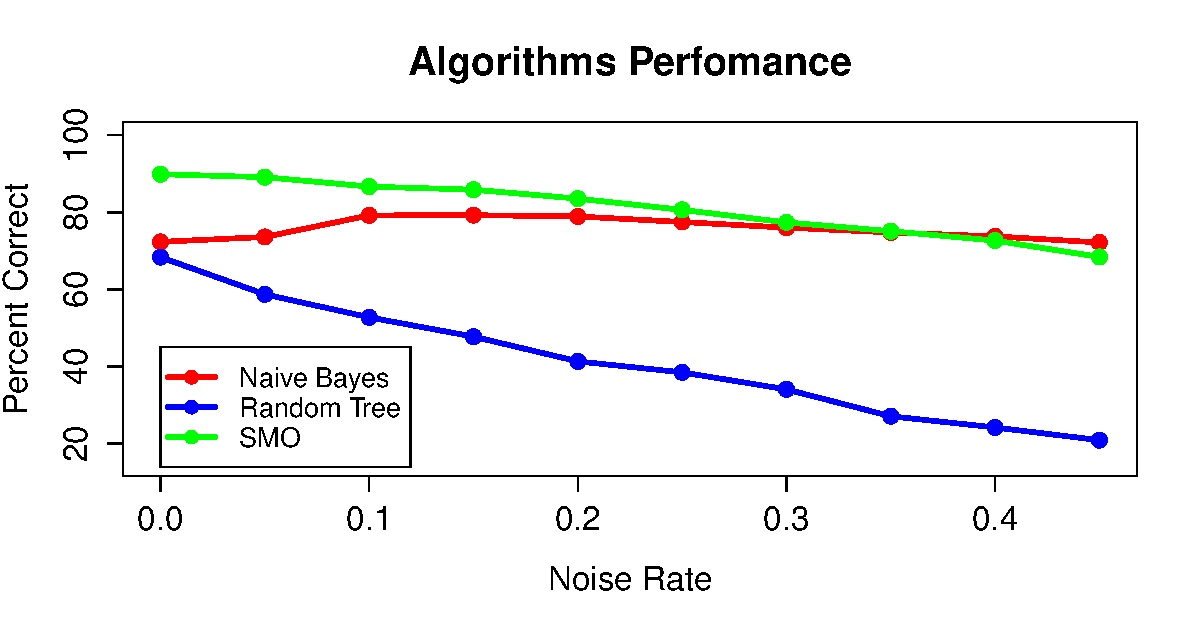
\includegraphics[width=\textwidth]{graphics/perfomance1.pdf}

\end{document}